\section{Computation architectures}
\label{sec:comparch}
Normally computations are preformed on a computers Central Processing Unit - a CPU.
A CPU is often fastest for everyday task and calculations.
The CPU consist of only a few cores which are highly optimized for sequential serial processing.\citep{whatisgpu}
But in recent years developers and sciencetist seem to have developed at interest for preforming calculations on Dedicated Graphic Processing Units.\citep{gpurise}
This is a whole other architechture which normally only was used for graphics processing but with some problems it seems that one coud utilise a GPU for General Purpose GPU compution - GPGPU, with an performance inprovement over a CPU.
In the following text we explore the possiblities that a GPU architecture offers.

GPUs are very common in desktop and laptops. \citep{STEAMHW}
GPUs are commonly used in the private and professional world, for computer gaming and accelerating graphic intensive programs such as Adobe Photoshop and 3D modelling tools. \citep{NVIDIAADOBE}
Their architecture can also be used for advantageously for certain types of computations, primarily computations which can be done in parallel. 
An example of this can be calculating different properties of the pixels on a screen. 
The screen can then be divided into different sections and the computations for each section is divided over the GPU internally.
This is possible because the specific calculations do not require results from the other calculations.
Unlike the cores in the CPU the cores in the GPU are not optimized for sequential serial processing, instead its cores are designed to handle multiple tasks at once. 
As such running sequential code on the CPU will be more efficient, where as more compute-intensive functions may be better suited for the GPU.\citep{NvidiaGPGPU}
The before mentioned example with pixels can be viewed as a matrix being divided into sections, so the same method of parallelised workflow can be applied for much liniar algebra expecially many operations on matrices where the problem can be split to nondependent subproblems.

\begin{figure}[h!]
\centering
 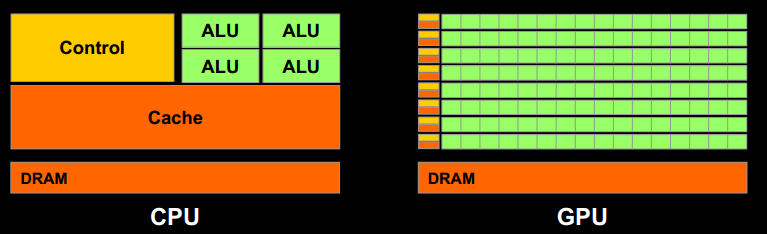
\includegraphics[width=1\textwidth]{figures/GPUCPUimage.png} % trim=4.85cm 15cm 0.85cm 1cm
\caption{A basic representation of the Transistor allocation on a GPU compared to a CPU}\label{image:GPUCPUimage}\citep{NvidiaCUDASeminar}
\vspace{-15pt}
\end{figure}

A simple representational comparison of a CPU - and a GPU's transistor usage is shown in \myref{image:GPUCPUimage}.
The GPU consists of more less powerful cores where as the CPU consists of fewer more powerful ones, the greater amount of cores allows for more computation power.
But to be able to utilise this computation power a problem must able to be split up, so many or all the cores in the GPU is used.
As of Q1 2015 an example of a modern high end desktop CPU is the Intel Haswell core i7 5960X which has 8 cores. \citep{puget}
A contemporary high end GPU is the NVIDIA GTX 980 which has 2048 CUDA cores. \citep{techpowerup,gtx980}
Due to their architectural differences the GPU allows for about 12 times more operations per second.

This makes the GPU particularly useful for large and complex computation, even some which are not graphical, if it is possibly to distribute the workload among the GPU cores.
But the GPU has an overhead.
This means that moving computations to the GPU cost a lot af time compared to running the computations on the CPU.
Therefore one has to reach a certian size of computation, before the advantage of parallel GPU computations exceeds the cost of transfering calculations onto the GPU.
To illustrate this problem as well a estimate an approximate computaion size where the GPU is advantageous we have written some test problems, which preforms different opreations on all elements in a matrix. 

\subsection{GPU and CPU computations comparison}
In this section we set up some calculations which can be split up in parallel problems to take advantages of the GPU arcitechture described in \myref{app:gpuoverhead}.
We will write and run a program written i regular C and write an equilent in CUDA which utilize the GPU for computations.
With these programs, we will then scale the size of the problems and compare the execution time for the C programs and the CUDA programs, to estimate where the threshold for computations on GPU lies.
We have chosen our testcase to be a matrix opration, more precisely the  Hadamard product

\begin{figure}[h!]
\centering
 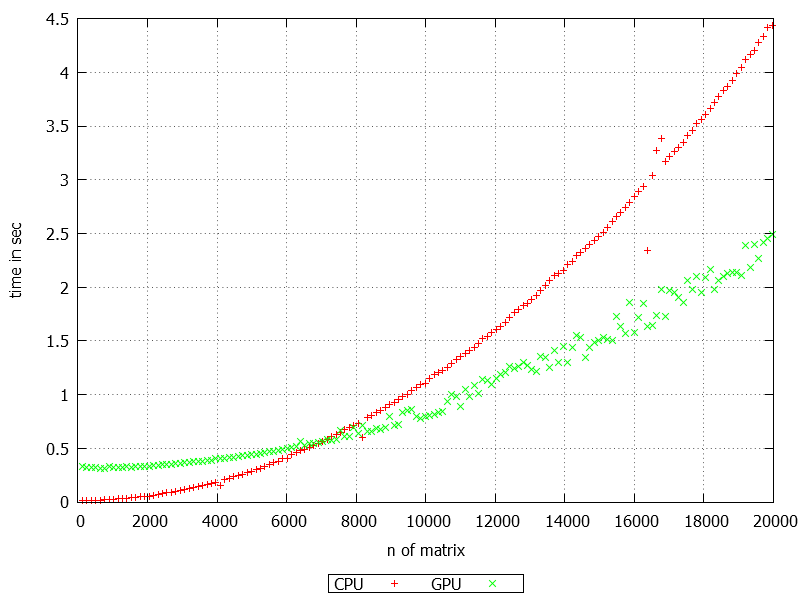
\includegraphics[width=1\textwidth]{figures/benchmark.png} % trim=4.85cm 15cm 0.85cm 1cm
\caption{A becnhmark of preforming 7 opertions on each element in a square matrix with size n on respectively a CPU and a GPU.}\label{image:benchmark}
\vspace{-15pt}
\end{figure}
